% 同一教学规则的四种输入与当前样本；正文宽度设计。
\begin{tikzpicture}[foundation picture]
 \path[use as bounding box] (0,-5) rectangle (112,60);
 \node at (25,46) {$f=1+2x_1+4x_2$};
 \node at (7,36) {输入}; \node at (25,36) {分数}; \node at (41,36) {动作};
 \foreach \y/\xone/\xtwo/\score/\result in {28/0/0/1/放行,20/1/0/3/放行,12/0/1/5/放行,4/1/1/7/隔离}{
  \node at (7,\y) {$(\xone,\xtwo)$};
  \node at (25,\y) {$\score$}; \node at (41,\y) {\result};
 }

 \node[inner sep=0pt] at (82,23) {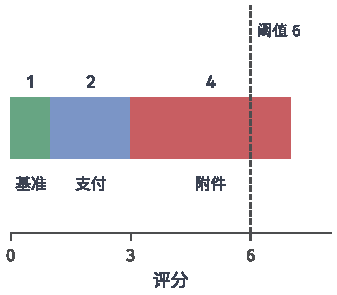
\includegraphics[width=57mm]{figures/02-foundations/03-trustworthiness/tikz/trust-global-local-explanation/trust-global-local-explanation.pdf}};
\node at (82,55) {当前邮件$(1,1)$};
\end{tikzpicture}